\documentclass{beamer}
\usepackage[utf8]{inputenc}


\usetheme{Madrid}
\usecolortheme{default}
\useinnertheme{circles}
\usepackage{tikz}
\setbeamercovered{dynamic}

\definecolor{Logo1}{rgb}{0.208, 0.2865, 0.373}
\definecolor{Logo2}{rgb}{0.000, 0.674, 0.863}

\setbeamercolor*{palette primary}{bg=Logo1, fg=white}
\setbeamercolor*{palette secondary}{bg=Logo2, fg=white}
\setbeamercolor*{palette tertiary}{bg=white, fg=Logo1}
\setbeamercolor*{palette quaternary}{bg=Logo1,fg=white}
\setbeamercolor{structure}{fg=Logo1} % itemize, enumerate, etc
\setbeamercolor{section in toc}{fg=Logo1} % TOC sections

%------------------------------------------------------------
%This block of code defines the information to appear in the
%Title page
\title{Сучасні методи управління проектами (Scrum, Kanban)}

%\subtitle{And its subtitle}

\author{Мнацаканов Антон}

\institute[КПІ] % (optional)
{
  Національний технічний університет України\\
  "Київський політехнічний інститут імені Ігоря Сікорського"
}

\date{\today}


%\logo{\includegraphics[height=.5cm]{logo-footer.png}}

%End of title page configuration block
%------------------------------------------------------------



%------------------------------------------------------------
%The next block of commands puts the table of contents at the 
%beginning of each section and highlights the current section:

\AtBeginSection[]
{
  \begin{frame}
    \frametitle{Зміст}
    \tableofcontents[currentsection]
  \end{frame}
}
%------------------------------------------------------------
\usepackage{array}
\usepackage{colortbl}
\usepackage{hhline}
\usepackage[english,russian,ukrainian]{babel}
%\usepackage{fourier}
\usepackage{lmodern}


\usepackage{ textcomp }
\usepackage{ eqnarray }
\usepackage{ txfonts }
\usepackage{hyperref}

\begin{document}

%The next statement creates the title page.
\frame{\titlepage}


%---------------------------------------------------------
%This block of code is for the table of contents after
%the title page
\begin{frame}
\frametitle{Зміст}
\tableofcontents
\end{frame}
%---------------------------------------------------------



%-------------------------------------------------------




\section{Scrum}
\begin{frame}
\frametitle{Scrum}
\center{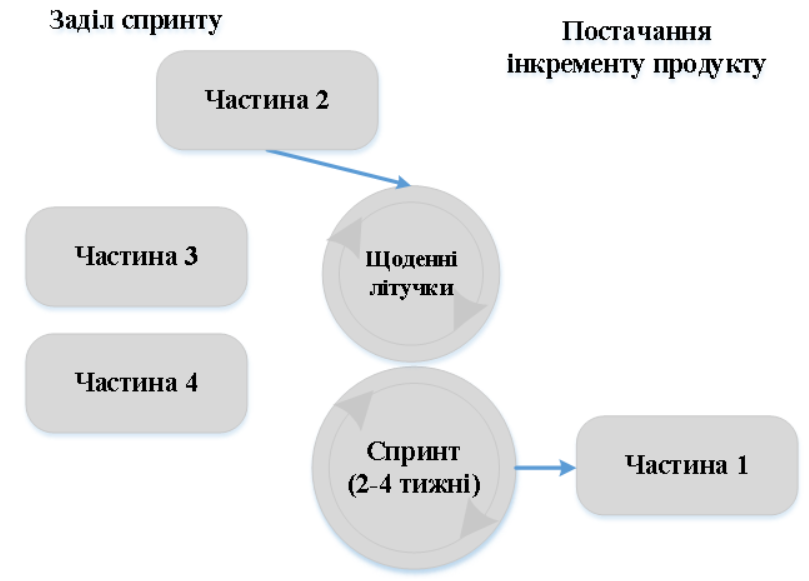
\includegraphics[width=0.5\linewidth]{3.png}}\\
Scrum розбиває проект на частини, які відразу можуть бути використані Замовником для отримання цінності, які називаються заділами продуктів (product backlog). Потім ці частини розбиваються за пріоритетом власником продукту – представником замовника в команді. 
\end{frame}


\section{}
\begin{frame}
\frametitle{Сильні та слабкі сторони Scrum }
Scrum був розроблений для проектів, в яких необхідні «швидкі перемоги» в поєднанні з толерантністю до змін. Крім того, цей фреймворк підходить для ситуацій, коли не всі члени команди мають достатній досвід в тій сфері, в якій реалізується проект – постійні комунікації між членами командами дозволяють зменшити недостачу досвіду або кваліфікації одних співробітників за рахунок більш кваліфікованих колег.\\ 

Scrum дуже вимогливий до команди проекту. Вона повинна бути невеликою (5-9 чоловік) і кросфункціональною – тобто члени команди повинні володіти більш ніж однієї компетенцією, необхідної для реалізації проекту. Наприклад розробник програмного забезпечення повинен володіти знаннями в тестуванні і бізнес-аналітиці. Робиться це для того, щоб частина команди не «простоювала» на різних етапах проекту, а також для того, щоб співробітники могли допомагати і підміняти один одного.
\end{frame}






\section{Lean}
\begin{frame}
\frametitle{Lean}
\center{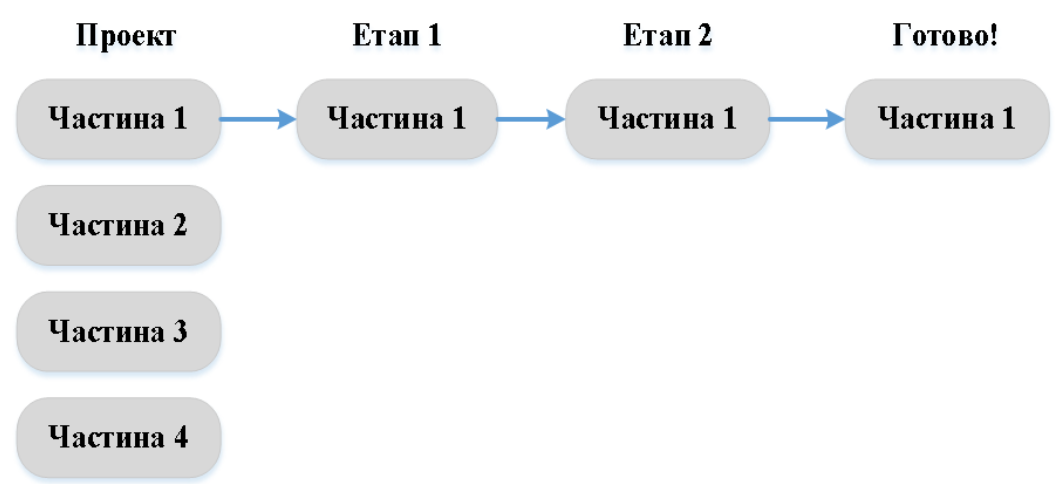
\includegraphics[width=0.6\linewidth]{4.png}}\\
  Agile говорить нам, що необхідно розбивати на невеликі керовані пакети робіт, але нічого не говорить про те, як управляти розробкою цього пакету. Scrum пропонує нам свої процеси і процедури. Lean ж, в свою чергу, додає до принципів Agile схему потоку операцій (workflow) для того, щоб кожна з ітерацій виконувалася однаково якісно.
\end{frame}



\section{Kanban}
\begin{frame}
\frametitle{Kanban}
\center{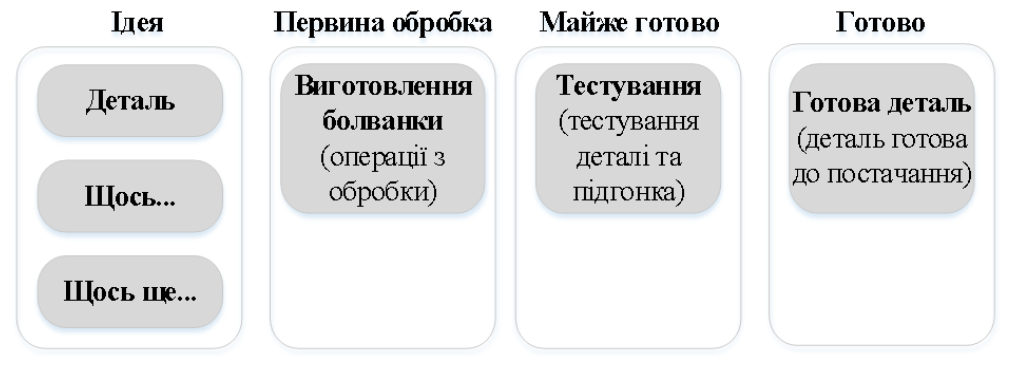
\includegraphics[width=0.6\linewidth]{5.png}}\\
Lean виглядає трохи абстрактним сам по собі, але в комбінації з Kanban його стає набагато простіше використовувати для побудови власної системи управління проектами. Створений інженером компанії Toyota Taiichi Ono в 1953 році, Kanban дуже схожий на схему промислового виробництва. На вході в цей процес потрапляє шматочок металу, а на виході виходить готова деталь. Також і в Kanban, інкремент продукту передається вперед з етапу на етап, а в кінці виходить готовий до постачання елемент.
\end{frame}


\section{}
\begin{frame}
\frametitle{Сильні та слабкі сторони Kanban }


Як і Scrum, Kanban добре підходить для досить згуртованої команди з хорошою комунікацією. Але на відміну від Scrum, в Kanban немає встановлених чітких дедлайнів, що добре підходить для мотивованих і досвідчених команд.\\ 

 

Kanban найкраще підходить для команд, навички членів яких перетинаються один з одним. Таким чином вони можуть допомагати один одному долати труднощі при вирішенні завдань. Без цього Kanban буде не такий ефективний, як міг би бути. Kanban краще підходить в випадках коли немає жорстких дедлайнів. Для жорстких дедлайнів краще підходить класичний підхід або Scrum.
\end{frame}



\section{Six Sigma}
Методологія що використовується у корпоративному менеджменті для вдосконалення виробництва та усунення дефектів. Стратегічний підхід до вдосконалення бізнесу, в рамках якого проводяться заходи зі знаходження і виключення причин помилок або дефектів у бізнес-процесах, шляхом зосередження на тих вихідних параметрах, які є критично важливими для споживача.
 
 
 
https://sgv.in.ua/off-lifaq/25-suchasni-metodi-upravlinnya-proektami

 
 


 
\begin{frame}
\frametitle{}
\begin{center}
Дякую за увагу!
\end{center}
\end{frame}














\end{document}